%%%%%%%%%%%%%%%%%%%%%%%%%%%%% Define Article %%%%%%%%%%%%%%%%%%%%%%%%%%%%%%%%%%
\documentclass[conference]{IEEEtran}
%%%%%%%%%%%%%%%%%%%%%%%%%%%%%%%%%%%%%%%%%%%%%%%%%%%%%%%%%%%%%%%%%%%%%%%%%%%%%%%

%%%%%%%%%%%%%%%%%%%%%%%%%%%%% Using Packages %%%%%%%%%%%%%%%%%%%%%%%%%%%%%%%%%%
\usepackage{geometry}
\usepackage{graphicx}
\usepackage{amssymb}
\usepackage{amsmath}
\usepackage{amsthm}
\usepackage{empheq}
\usepackage{mdframed}
\usepackage{booktabs}
\usepackage{lipsum}
\usepackage{graphicx}
\usepackage{color}
\usepackage{psfrag}
\usepackage{pgfplots}
\usepackage{bm}
\usepackage[spanish]{babel}
\usepackage[utf8]{inputenc} % Codificación UTF-8
\usepackage{amsmath}        % Soporte para ecuaciones matemáticas
\usepackage{graphicx}       % Manejo de imágenes
\usepackage{hyperref}       % Hipervínculos
\usepackage{caption}        % Formato para figuras
\usepackage{multirow}
\usepackage{subcaption}
\usepackage{bookmark}

% %%%%%%%%%%%%%%%%%%%%%%%%%%%%%%%%%%%%%%%%%%%%%%%%%%%%%%%%%%%%%%%%%%%%%
% %% SE ELIMINAN LAS LÍNEAS DE biblatex PORQUE SON INCOMPATIBLES %%%%%%%
% \usepackage{biblatex}
% \usepackage{csquotes}
% \renewcommand*{\bibfont}{\footnotesize}
% \setlength{\biblabelsep}{\labelsep}
% \setlength{\bibitemsep}{\IEEEbibitemsep}
% \addbibresource{refabetsito.bib}
% %%%%%%%%%%%%%%%%%%%%%%%%%%%%%%%%%%%%%%%%%%%%%%%%%%%%%%%%%%%%%%%%%%%%%

%%%%%%%%%%%%%%%%%%%%%%%%%%%%%%%%%%%%%%%%%%%%%%%%%%%%%%%%%%%%%%%%%%%%%%%%%%%%%%%

% Other Settings

%%%%%%%%%%%%%%%%%%%%%%%%%% Page Setting %%%%%%%%%%%%%%%%%%%%%%%%%%%%%%%%%%%%%%%
\geometry{a4paper, margin=1in}

%%%%%%%%%%%%%%%%%%%%%%%%%% Define some useful colors %%%%%%%%%%%%%%%%%%%%%%%%%%
\definecolor{ocre}{RGB}{243,102,25}
\definecolor{mygray}{RGB}{243,243,244}
\definecolor{deepGreen}{RGB}{26,111,0}
\definecolor{shallowGreen}{RGB}{235,255,255}
\definecolor{deepBlue}{RGB}{61,124,222}
\definecolor{shallowBlue}{RGB}{235,249,255}
%%%%%%%%%%%%%%%%%%%%%%%%%%%%%%%%%%%%%%%%%%%%%%%%%%%%%%%%%%%%%%%%%%%%%%%%%%%%%%%

%%%%%%%%%%%%%%%%%%%%%%%%%% Define an orangebox command %%%%%%%%%%%%%%%%%%%%%%%%
\newcommand\orangebox[1]{\fcolorbox{ocre}{mygray}{\hspace{1em}#1\hspace{1em}}}
%%%%%%%%%%%%%%%%%%%%%%%%%%%%%%%%%%%%%%%%%%%%%%%%%%%%%%%%%%%%%%%%%%%%%%%%%%%%%%%

%%%%%%%%%%%%%%%%%%%%%%%%%%%% English Environments %%%%%%%%%%%%%%%%%%%%%%%%%%%%%
\newtheoremstyle{mytheoremstyle}{3pt}{3pt}{\normalfont}{0cm}{\rmfamily\bfseries}{}{1em}{{\color{black}\thmname{#1}~\thmnumber{#2}}\thmnote{\,--\,#3}}
\newtheoremstyle{myproblemstyle}{3pt}{3pt}{\normalfont}{0cm}{\rmfamily\bfseries}{}{1em}{{\color{black}\thmname{#1}~\thmnumber{#2}}\thmnote{\,--\,#3}}
\theoremstyle{mytheoremstyle}
\newmdtheoremenv[linewidth=1pt,backgroundcolor=shallowGreen,linecolor=deepGreen,leftmargin=0pt,innerleftmargin=20pt,innerrightmargin=20pt,]{theorem}{Theorem}[section]
\theoremstyle{mytheoremstyle}
\newmdtheoremenv[linewidth=1pt,backgroundcolor=shallowBlue,linecolor=deepBlue,leftmargin=0pt,innerleftmargin=20pt,innerrightmargin=20pt,]{definition}{Definition}[section]
\theoremstyle{myproblemstyle}
\newmdtheoremenv[linecolor=black,leftmargin=0pt,innerleftmargin=10pt,innerrightmargin=10pt,]{problem}{Problem}[section]
%%%%%%%%%%%%%%%%%%%%%%%%%%%%%%%%%%%%%%%%%%%%%%%%%%%%%%%%%%%%%%%%%%%%%%%%%%%%%%%

%%%%%%%%%%%%%%%%%%%%%%%%%%%%%%% Plotting Settings %%%%%%%%%%%%%%%%%%%%%%%%%%%%%
\usepgfplotslibrary{colorbrewer}
\pgfplotsset{width=8cm,compat=1.9}
%%%%%%%%%%%%%%%%%%%%%%%%%%%%%%%%%%%%%%%%%%%%%%%%%%%%%%%%%%%%%%%%%%%%%%%%%%%%%%%

%%%%%%%%%%%%%%%%%%%%%%%%%%%%%%% Title & Author %%%%%%%%%%%%%%%%%%%%%%%%%%%%%%%%
\author{\IEEEauthorblockN{Daniel Fernando Aranda Contreras, Dairo Alexander Lobo Moreno,\\ Yulieth Valentina Portilla Jaimes}
\IEEEauthorblockA{Escuela E3T, Universidad Industrial de Santander\\
Correo electrónico: \{daniel2221648, dairo2221123, yulieth2221136\}@correo.uis.edu.co}}

%%%%%%%%%%%%%%%%%%%%%%%%%%%%%%%%%%%%%%%%%%%%%%%%%%%%%%%%%%%%%%%%%%%%%%%%%%%%%%%
    
\begin{document}
    % Título
    \title{Control MPPT en Convertidor Boost para una carga 8540 [W]}
    \maketitle
    % Resumen
    % Palabras clave
    \begin{IEEEkeywords}
        Control MPPT, Convertidor Boost, Panel Solar, Módulo Fotovoltaico, Dimensionamiento de componentes, Arreglo fotovoltaico, Simulink, Rizado.
    \end{IEEEkeywords}

\section{Resumen}
En este laboratorio se trabajó con la simulación de un sistema fotovoltaico que utiliza un convertidor boost para alimentar una carga residencial de 120 Vrms. Con ayuda de la herramienta MATLAB/Simulink, se usó el módulo fotovoltaico A10 Green A10J-M60-240. En base a los datos de este, se definió la conexión serie-paralelo para alcanzar su potencia máxima, dada en 8.5 kW. Con el fin de garantizar niveles adecuados de tensión y rizado, se hicieron los cálculos pertinentes que debía cumplir la electrónica de potencia. De la mano de est c    os cálculos se hallaron los valores principales del convertidor, como la relación de conversión, el inductor y los capacitores de entrada y salida, considerando el rizado permitido y manteniendo la operación en conducción continua. La carga conectada al bus de 200 V se representó tanto como resistencia equivalente como potencia constante. Con este modelo se logró establecer la base del sistema, que más adelante permitirá integrar un algoritmo MPPT y analizar su comportamiento frente a variaciones en las condiciones de operación.



\section{Introducción}
Con la creciente integración de \textbf{generación fotovoltaica}, para los usuarios de las viviendas esto se ha convertido en una opción muy atractiva ya que reduce el impacto ambiental y aprovecha una energía más limpia. La cantidad de potencia que entrega un panel solar se ve afectada por factores como la \textbf{irradiancia}, la \textbf{temperatura} y el punto de operación sobre la curva $I-V$. Una operación lejos del punto de máxima potencia (\textbf{MPP}) genera pérdidas que reducen el aprovechamiento de la energía disponible.

Entonces, el método que se usa para evitar esto es contar con una etapa de conversión que adapte la tensión de los paneles a un nivel adecuado para la carga. Por ello se usa un \textbf{convertidor boost} (elevador) que se modela como una planta; con ayuda de él se eleva la tensión del arreglo fotovoltaico hasta un bus de 200 V en corriente continua. Desde allí, mediante un \textbf{inversor}, es posible alimentar una carga residencial de 120 Vrms. Para que este convertidor funcione de manera estable, es clave definir correctamente componentes como el \textbf{inductor} y los \textbf{capacitores}, considerando el rizado de corriente y tensión en el diseño.

\section{Datos del panel solar}
\begin{table}[ht!]
    \centering
    \caption{Parámetros del panel solar A10J-M60-240}
    \label{tab:panel_parameters}
    \begin{tabular}{|l|c|c|}
        \hline
        \textbf{Parámetro} & \textbf{Valor} & \textbf{Unidad} \\
        \hline
        Maximum Power ($P_{mp}$) & 240.5376 & W \\
        Cells per module ($N_{cell}$) & 60 & Unidad \\
        Open-circuit voltage ($V_{oc}$) & 36.84 & V \\
        Short-circuit current ($I_{sc}$) & 8.32 & A \\
        Voltage at maximum power point ($V_{mp}$) & 30.72 & V \\
        Current at maximum power point ($I_{mp}$) & 7.83 & A \\
        Temperature coefficient of $V_{oc}$ & -0.359 & \%/°C \\
        Temperature coefficient of $I_{sc}$ & 0.096995 & \%/°C \\
        \hline
    \end{tabular}
\end{table}





\section{Paso a paso del diseño}
\subsection{Elección del arreglo}
\begin{itemize}
    \item Tensión en el punto de máxima potencia (MPP) del arreglo:
    $$V_{mp,string} = N_{s} \cdot V_{mp,mod}$$
    \textbf{Datos obtenidos:} $V_{mp,string} = 184.32 \, \text{V}$
    
    \item Número de paneles en paralelo:
    $$N_{p} = \text{round}\left(\frac{P_{total}}{N_{s} \cdot P_{max,mod}}\right)$$
    \textbf{Datos obtenidos:} $N_{p} = 6$
    
    \item Potencia del arreglo:
    $$P_{arreglo} = N_{p} \cdot N_{s} \cdot P_{max,mod}$$
    donde $P_{arreglo} = 8659.3536 \, \text{W}$
    \textbf{Datos obtenidos:} $N_{s} = 6$
\end{itemize}

\subsection{Cálculo de la tensión en frío}
\begin{itemize}
    \item Tensión de circuito abierto ($V_{oc}$) del arreglo a temperatura T: 25 °C
    $$V_{oc,string}(T) = N_{s} \cdot V_{oc,STC} \cdot [1 + \beta_{Voc}(T-25^\circ C)]$$
    \textbf{Datos obtenidos:} $V_{oc,string}(T) = 221.04 \, \text{V}$
\end{itemize}

\subsection{Punto nominal del convertidor Boost}
\begin{itemize}
    \item Ciclo de trabajo (D) nominal del convertidor Boost:
    $$D = 1 - \frac{V_{in}}{V_{out}}$$
    \textbf{Datos obtenidos:} $D = 0.0784$
    
    \item Corriente promedio del inductor ($I_{L,avg}$):
    $$I_{L,avg} = \frac{P_{arreglo}}{V_{in}}$$
    \textbf{Datos obtenidos:} $I_{L,avg} = 46.98 \, \text{A}$
\end{itemize}


\subsection{Diseño del inductor}
Para garantizar que el convertidor opere en modo de conducción continua (CCM), se dimensionó el inductor a partir de la corriente media que circula por él y un criterio de rizado de aproximadamente el $10\%$. Con estos parámetros y la frecuencia de conmutación 20$kHs$, se aplicó la expresión del inductor de un convertidor tipo \textit{boost}.

\[
I_{L,\text{avg}} \approx \frac{P_{\text{array}}}{V_{in}},
\]
\[
\Delta I_L \approx 0.1\, I_{L,\text{avg}}.
\]
\[
L \approx \frac{V_{in} \cdot D}{\Delta I_L \, f_s}=0,154[mH]
\]

Finalmente, se comprobó que el valor calculado fuera mayor que el mínimo requerido para asegurar la operación en CCM,lo que asegura que la operación del convertidor se mantenga en CCM.
\[
L > L_{\min} \approx \frac{(1-D)^2 R}{2 f_s}
\]
\[
0,154 \,\text{mH} \; > \; 0,98 \,\text{mH}.
\]

\subsection{Cálculo de capacitores}

El capacitor se diseñó para suavizar la tensión en el arreglo fotovoltaico, que es limitar las variaciones de voltaje que aparecen debido al rizado de corriente del inductor.Ademas, este capacitor se seleccionó para limitar la  variación de tensión en el arreglo fotovoltaico a un valor pequeño del orden del $1\%$.De esta forma, se utilizó la relación:

\[
\Delta V_{pv,pp} \approx 1\%  \, V_{mp,string}.
\]
\[
C_{in} \gtrsim \frac{\Delta I_L}{8 \, f_s \, \Delta V_{pv,pp}},
\]
\[
C_{in} ={15,93\mu\text{F}}
\]

Mientras que el capacitor de salida se dimensionó para mantener estable la tensión del bus de continua y reducir el rizado a un valor aceptable, del orden 2 voltios.El cálculo se realizo a partir de :
\[
\Delta V_{dc,pp} \approx 2\ \mathrm{V}.
\]
La corriente en la salida, a partir de la potencia del arreglo, se calcula como:
\[
I_{out} \approx \frac{P}{V_{out}} = 43,296768\ \mathrm{A}
\]
\[
C_{out} \gtrsim \frac{I_{out} \cdot D}{f_s \, \Delta V_{dc,pp}}=84,86\mu\text{F}
\]

\subsection*{ Modelar la carga en el bus de 200 V}
La carga del convertidor se representó mediante una resistencia equivalente, este valor se define de manera que al aplicarle la tensión de salida$V_{out}$, la potencia disipada en la resistencia sea igual a la potencia máxima generada por el arreglo fotovoltaico ($P_{mpp,array}$). De esta forma, se emula el consumo del sistema con un modelo sencillo de analizar y se calculó a partir de la relación:

\[
R_{eq} = \frac{V_{out}^2}{P_{mpp,array}} = \; 4.62 \Omega
\]
\section{Montaje y simulación}
El montaje del convertidor se realizó en \textit{Simulink/Simscape Power Systems (SPS)}, empleando un modelo del arreglo fotovoltaico conectado a un convertidor tipo \textit{boost}. En la entrada se incluyó el modelo del \textit{PV Array} con condiciones de irradiancia de $1000 \,\text{W/m}^2$ y temperatura de $25^\circ \text{C}$, para el bus de salida se utilizó la resistencia equivalente calculada, junto con los valores comerciales seleccionados de inductor $L$, capacitores $C_{in}$ y $C_{out}$.  

El esquema de simulación incorporó también los bloques de conmutación con el diodo de potencia, así como las mediciones de tensión y corriente en los nodos de interés. Además, se añadió un bloque de control para generar el ciclo de trabajo ($D$) del interruptor, de modo que el convertidor pudiera operar en las condiciones calculadas.  


\begin{figure}[h!]
    \centering
    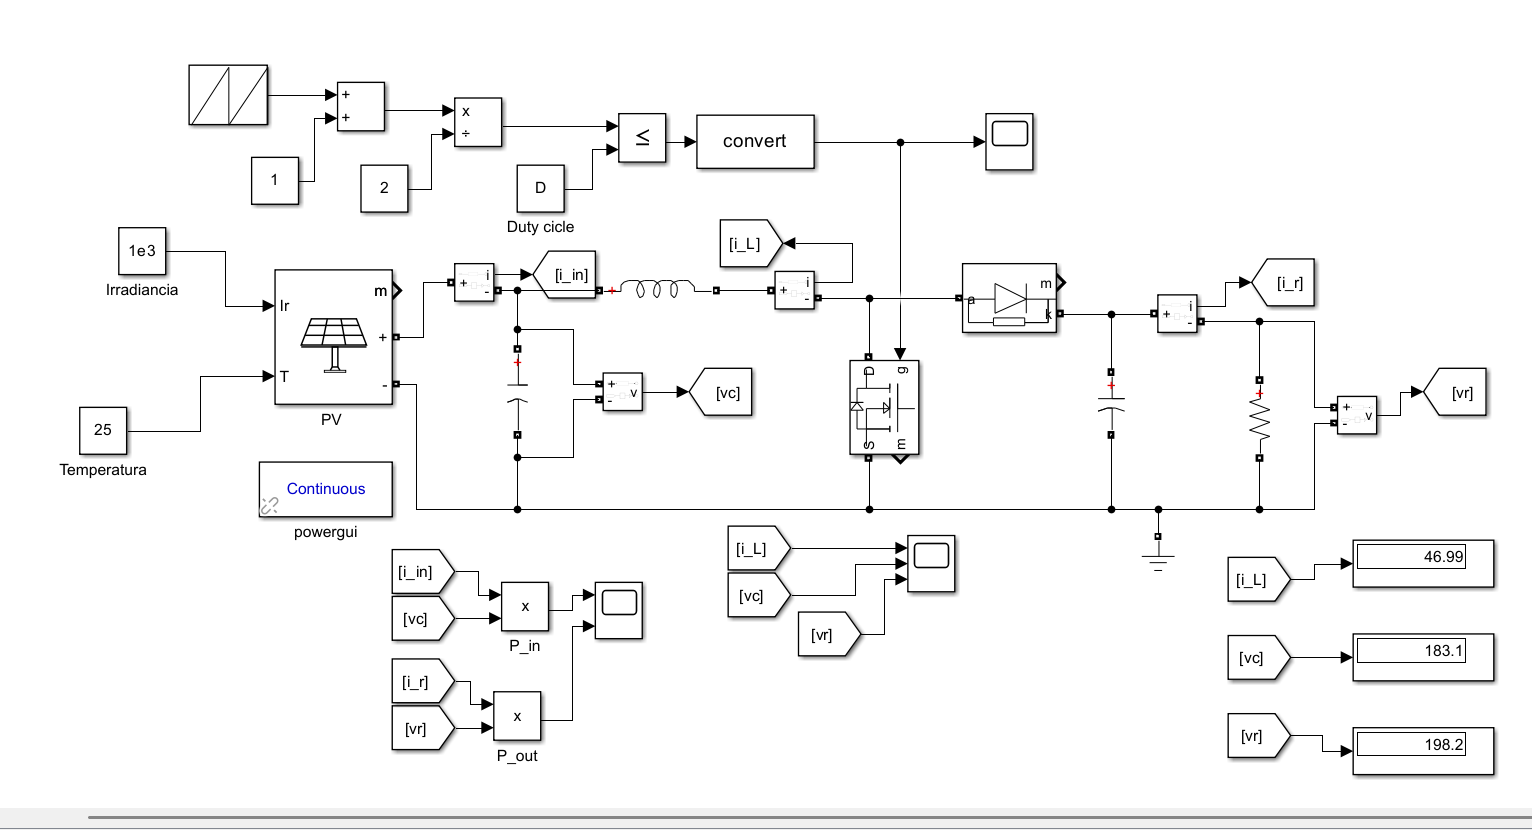
\includegraphics[width=1\linewidth]{fot/simulacion.png} % ajustar ancho si es necesario
    \caption{Simulación del sistema PV.}
    \label{fig:simulacion_pv}
\end{figure}


Ademas, para lograr resultados más realistas en el montaje y la simulación, los valores de diseño calculados para el inductor ($L$), los capacitores ($C_{\text{in}}$ y $C_{\text{out}}$), y la resistencia ($R_{\text{eq}}$) fueron sustituidos por valores comerciales. En el caso de los capacitores, se eligieron valores ligeramente superiores a los calculados para asegurar una mejor calidad de la salida al reducir el rizado de tensión, para el inductor, se seleccionó el valor comercial más cercano para mantener el correcto modo de conducción yfinalmente, se utilizó la resistencia comercial más cercana para representar con precisión la carga del sistema, como muestra la tabla a continuación.
 

\begin{table}[ht!]
\centering
\begin{tabular}{l c c}
\hline
Parámetro & Valor calculado & Valor comercial \\
\hline
$R_{eq}$   & $4,6\ \Omega$   & $4,7\ \Omega$ \\
$L$        & $153,8\ \mu$H   & $150\ \mu$H \\
$C_{in}$   & $15,9\ \mu$F    & $22\ \mu$F \\
$C_{out}$  & $84,9\ \mu$F    & $100\ \mu$F \\
\hline
\end{tabular}
\end{table}

De esta manera, la simulación permitió verificar el comportamiento dinámico del sistema y comprobar que la tensión de salida se estabilizara en torno a los $200 \,\text{V}$, cumpliendo con los criterios de diseño.  A continuación, se presentan las gráficas detalladas de las señales clave, incluyendo el ciclo de trabajo y los rizados de corriente y tensión, que demuestran el comportamiento de los componentes bajo condiciones de operación.

\subsection{Ciclo de Trabajo (D)}
La Figura presenta el ciclo de trabajo (D) aplicado al interruptor del convertidor, esta señal es vital, ya que controla la transferencia de energía y, por ende, la tensión de salida.

\begin{figure}[ht!]
    \centering
    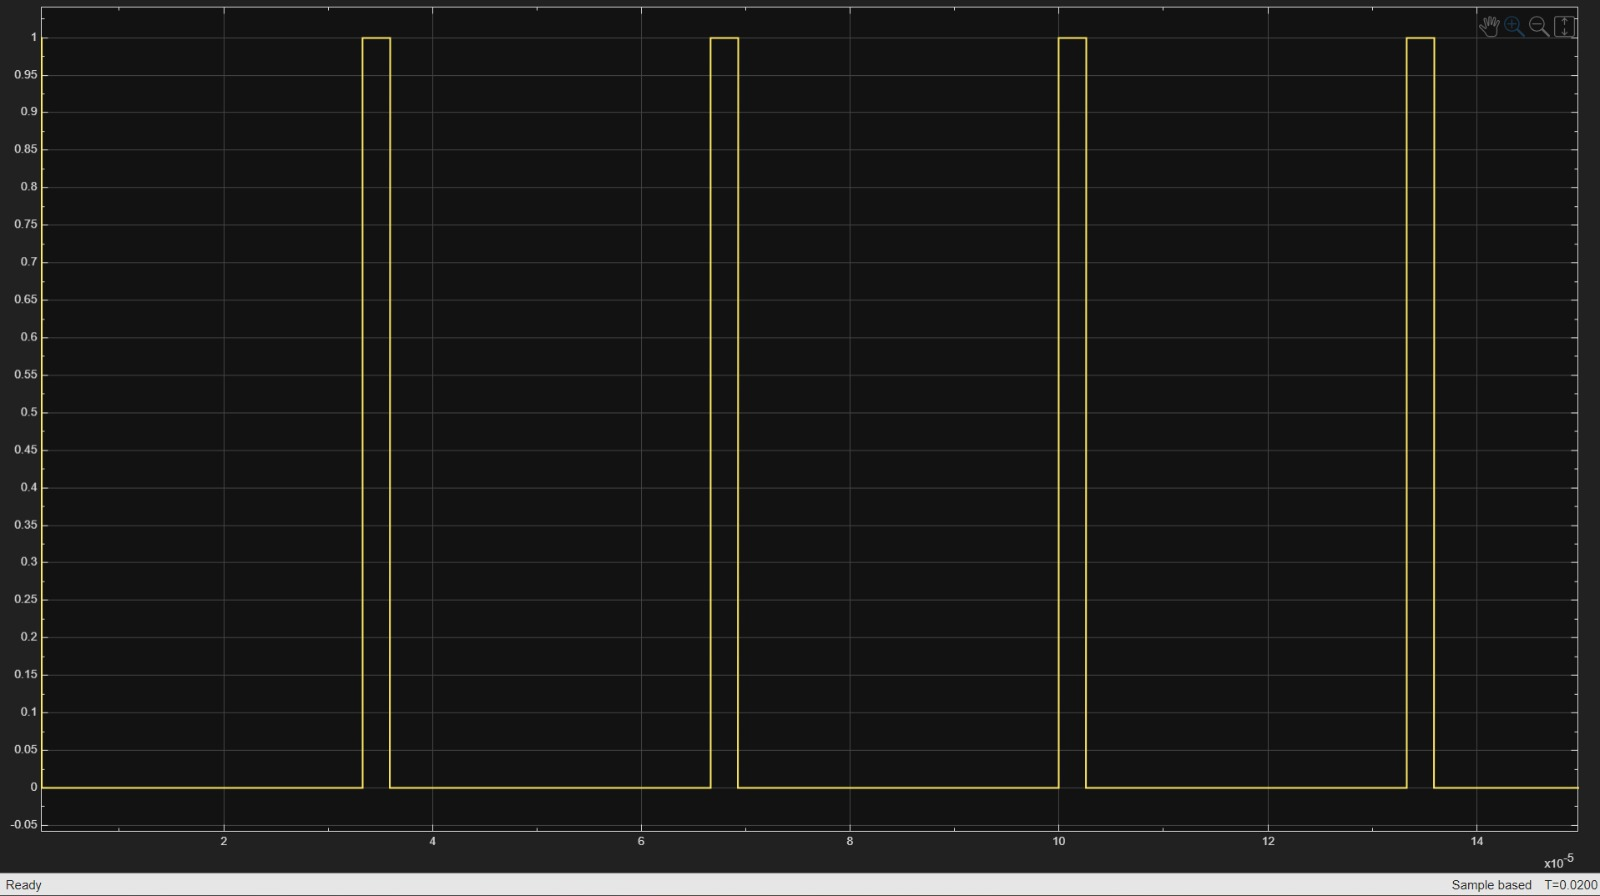
\includegraphics[width=0.9\linewidth]{fot/D.jpeg} 
    \caption{Ciclo de trabajo ($D$).}
    \label{fig:D}
\end{figure}

\subsection{Rizado de Corriente en el Inductor (i\_L)}

A continuación, se muestra el rizado de corriente en el inductor.Donde se logra observar que la corriente se mantiene dentro de los límites de diseño, confirmando el modo de conducción continua (CCM).

\begin{figure}[ht!]
    \centering
    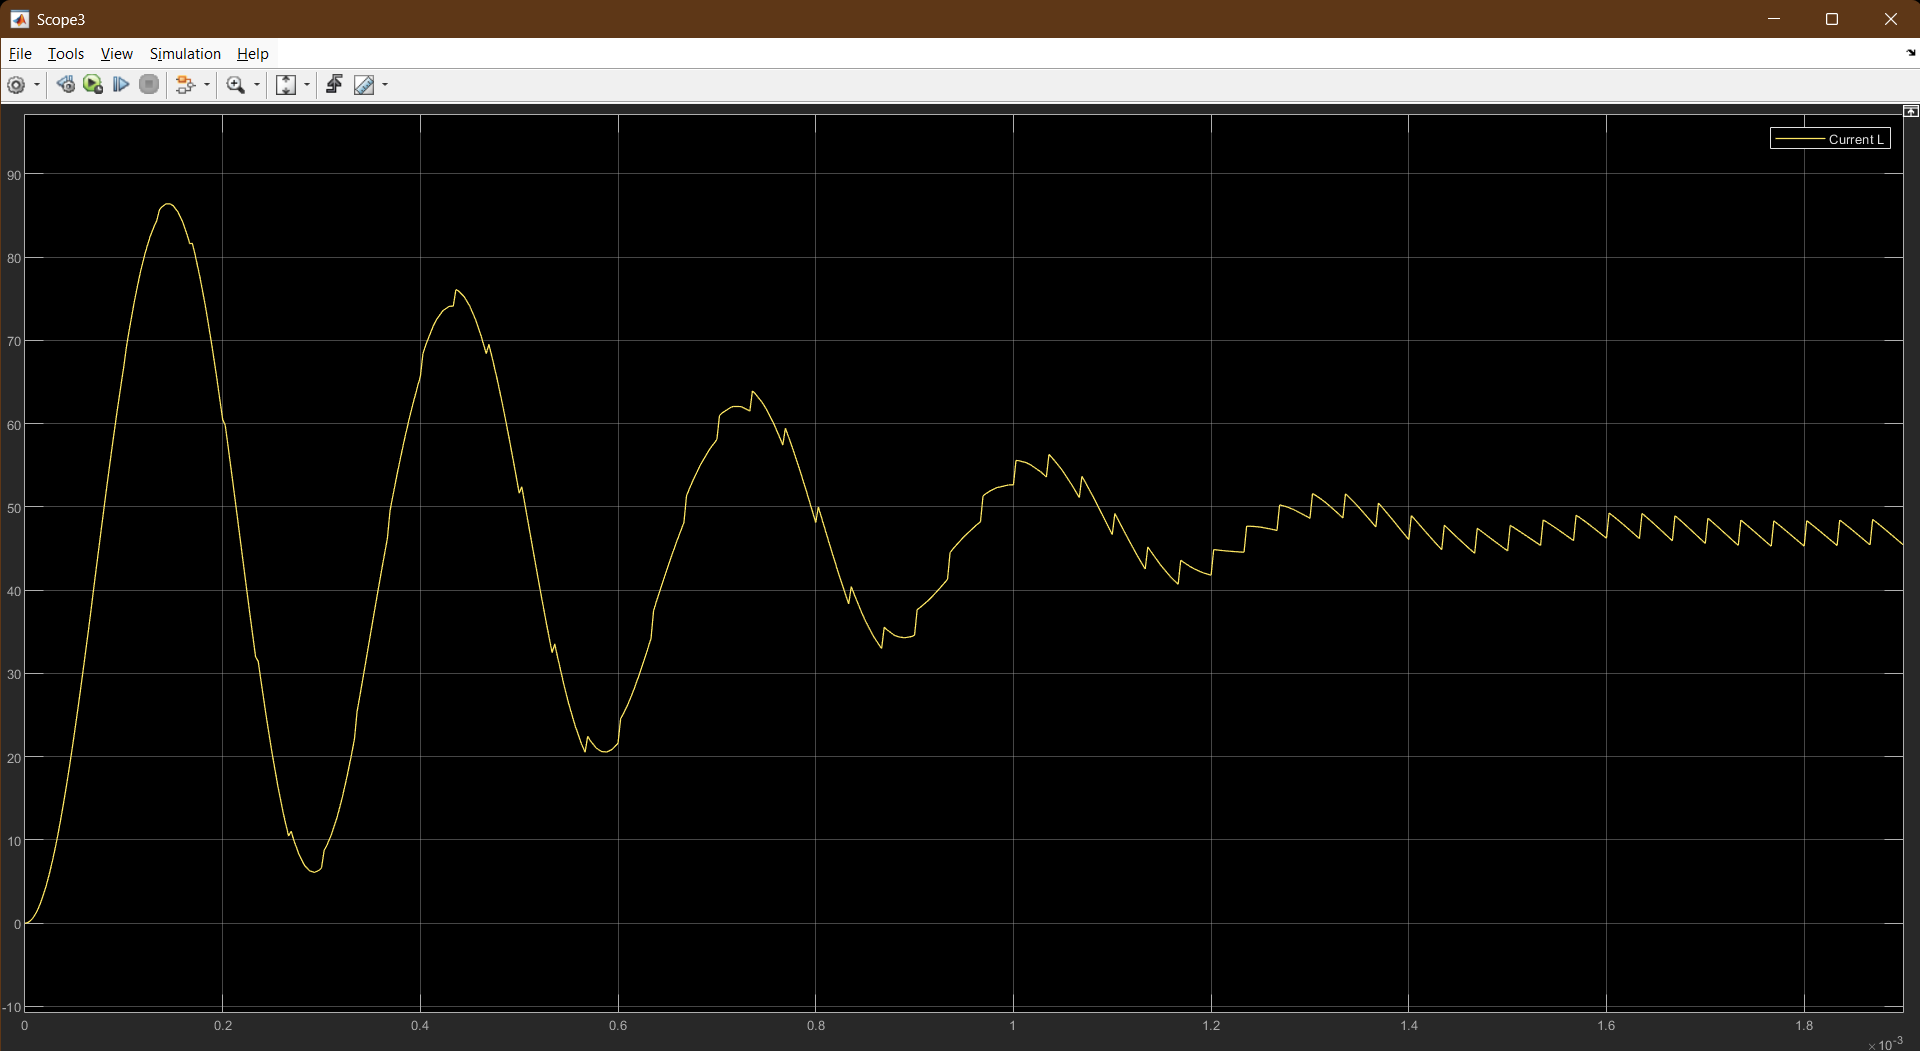
\includegraphics[width=0.9\linewidth]{fot/L.png} 
    \caption{Rizado de corriente en el inductor ($i_L$).}
    \label{fig:il}
\end{figure}


\subsection{Rizado de Tensión de Entrada (Vpv)}
En la Figura siguiente se visualiza el rizado de tensión en la entrada, este rizado es crucial para garantizar que el panel fotovoltaico opere de manera estable.


\begin{figure}[ht!]
    \centering
    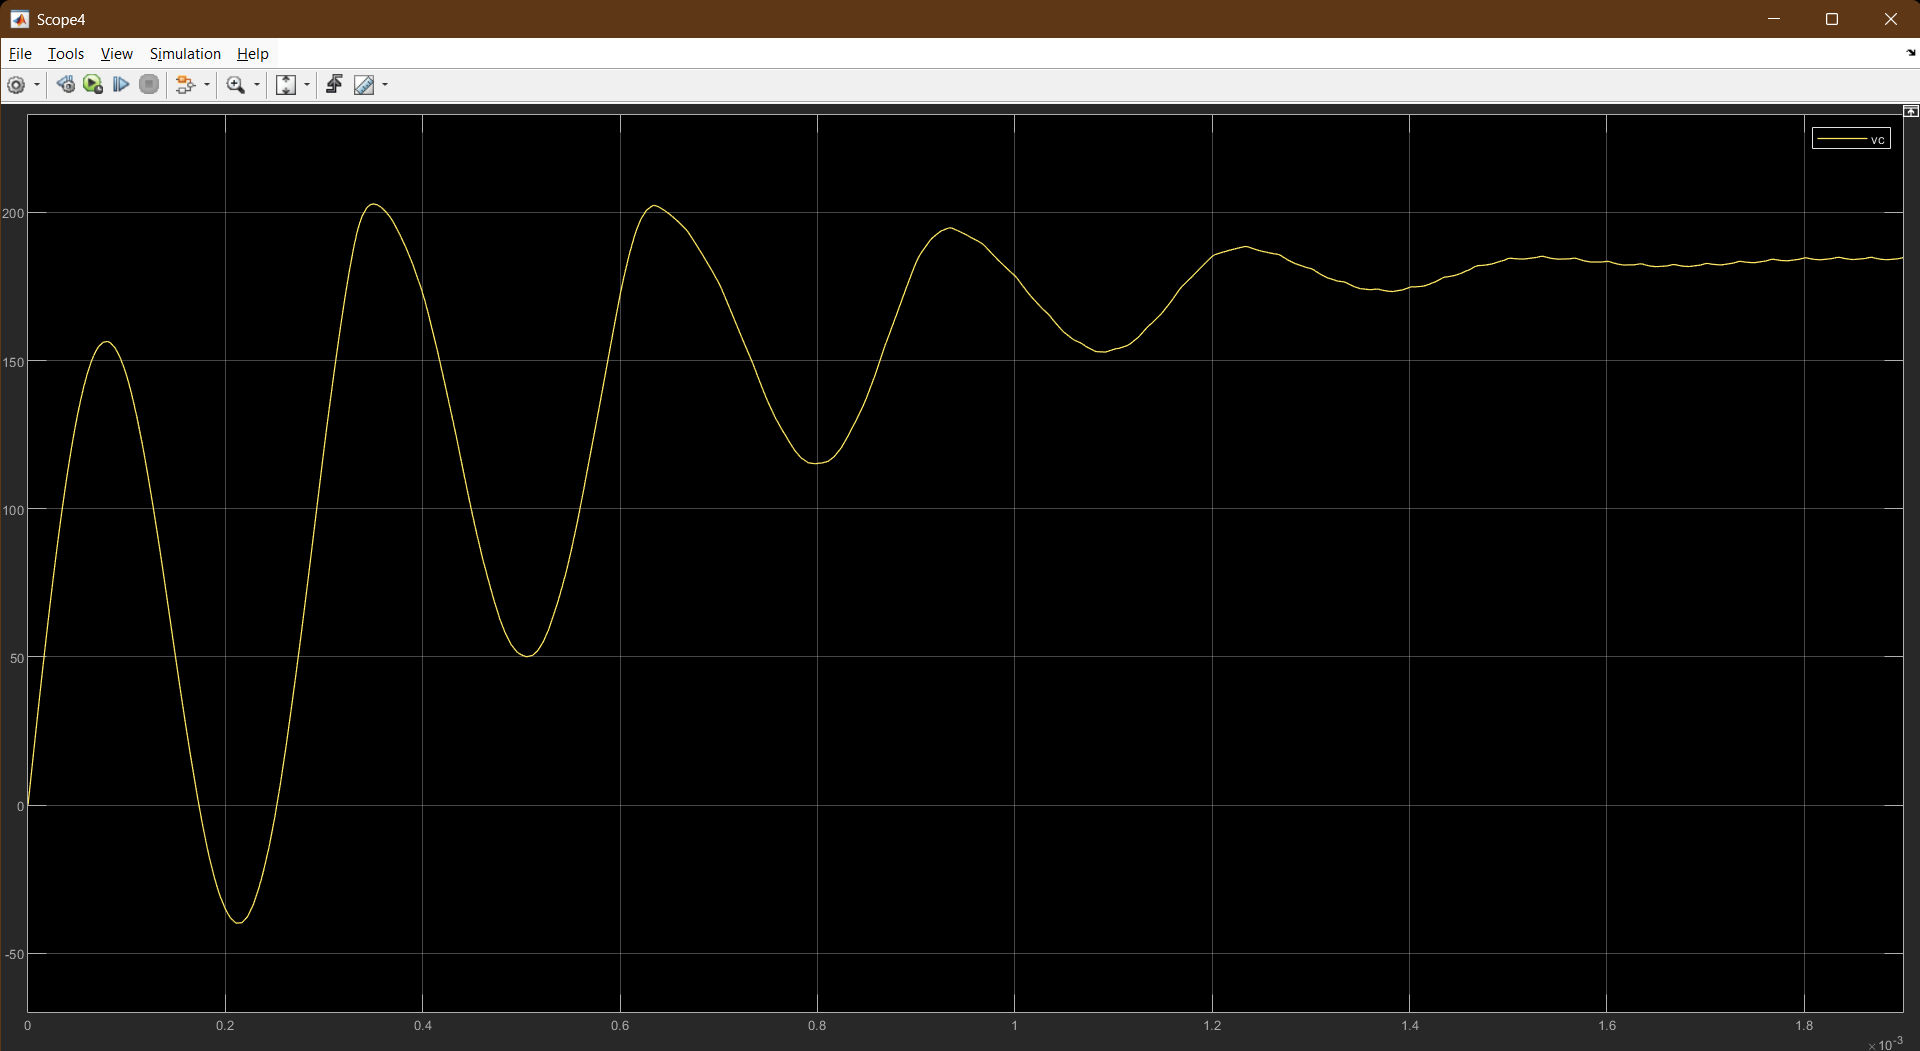
\includegraphics[width=0.9\linewidth]{fot/Cin.png} 
    \caption{Rizado de tensión en la entrada.}
    \label{fig:vin}
\end{figure}


\subsection{Rizado de Tensión en la salida}
Finalmente, la Figura siguiente ilustra el rizado de tensión en el capacitor de salida. Un bajo rizado aquí asegura una tensión de salida estable para la carga.

\begin{figure}[ht!]
    \centering
    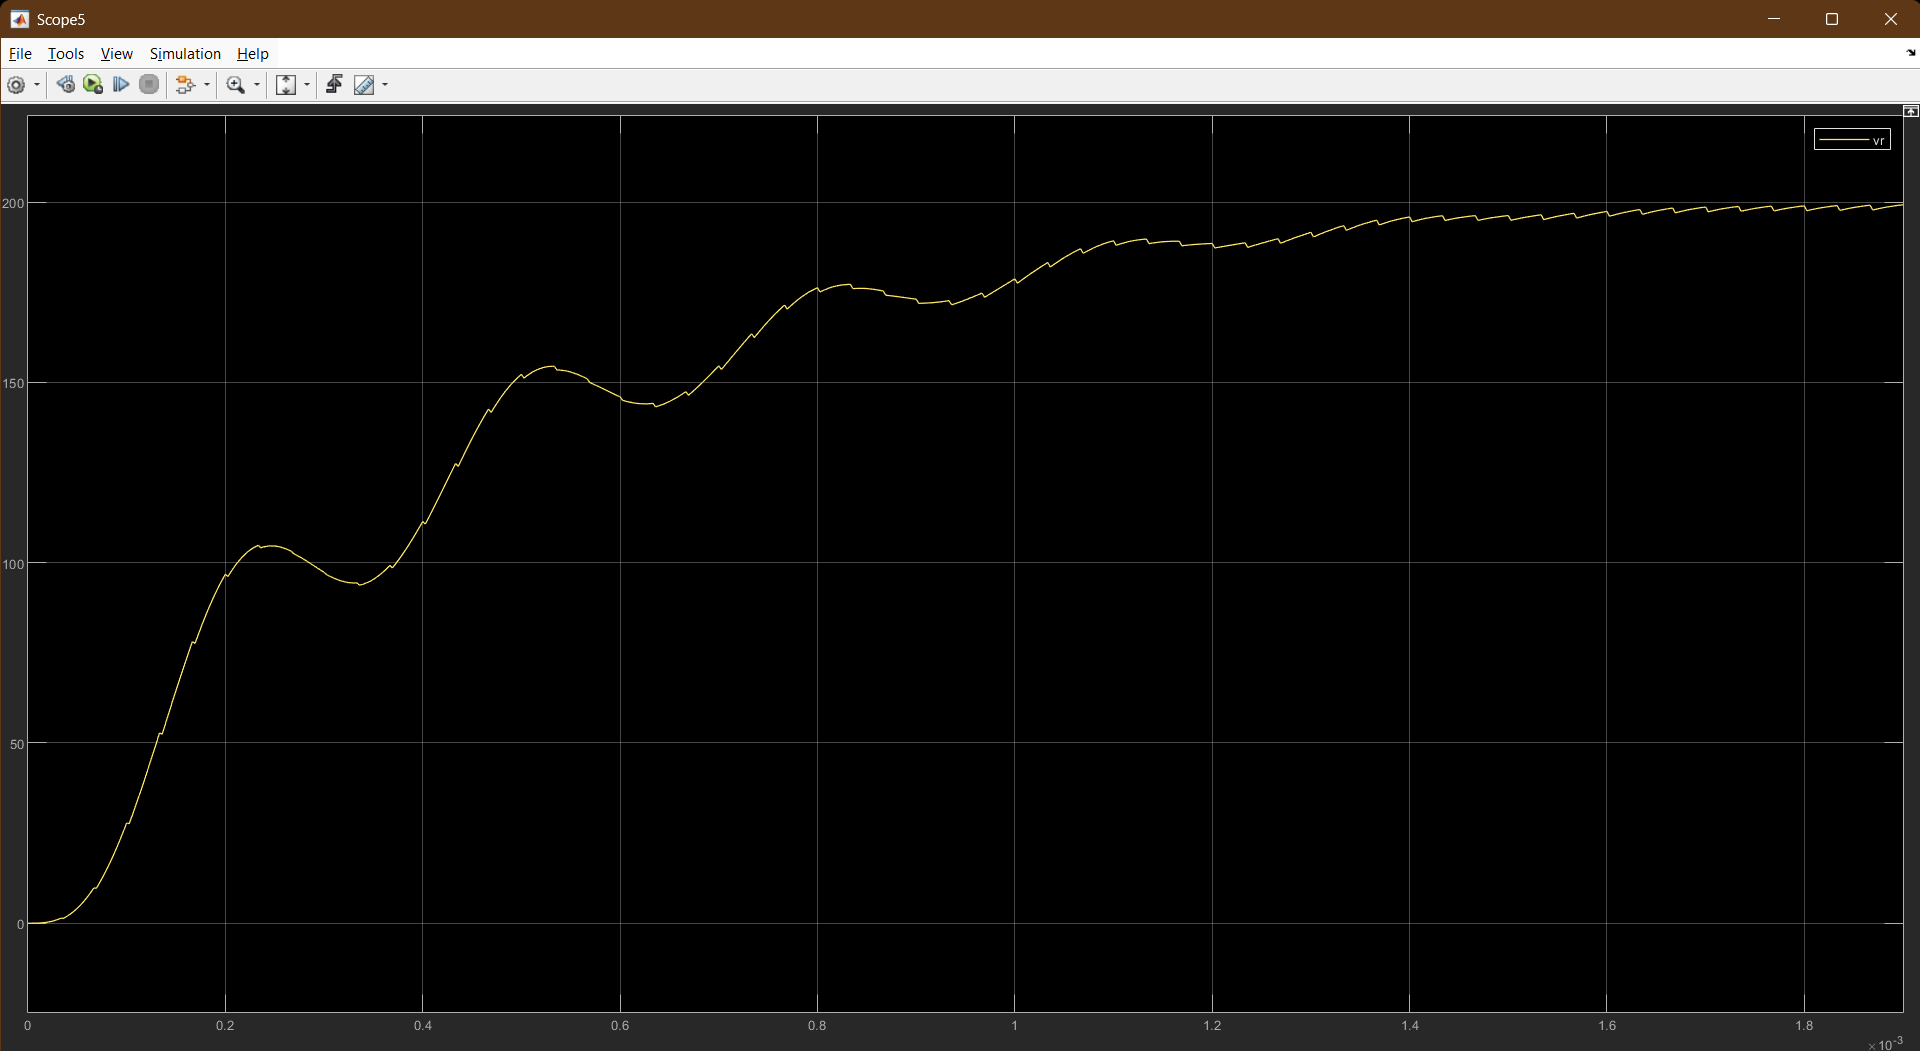
\includegraphics[width=0.9\linewidth]{fot/Cout.png} 
    \caption{Rizado de tensión en la salida.}
    \label{fig:vout}
\end{figure}

\section{Anexos}
\begin{figure}[ht!]
    \centering
    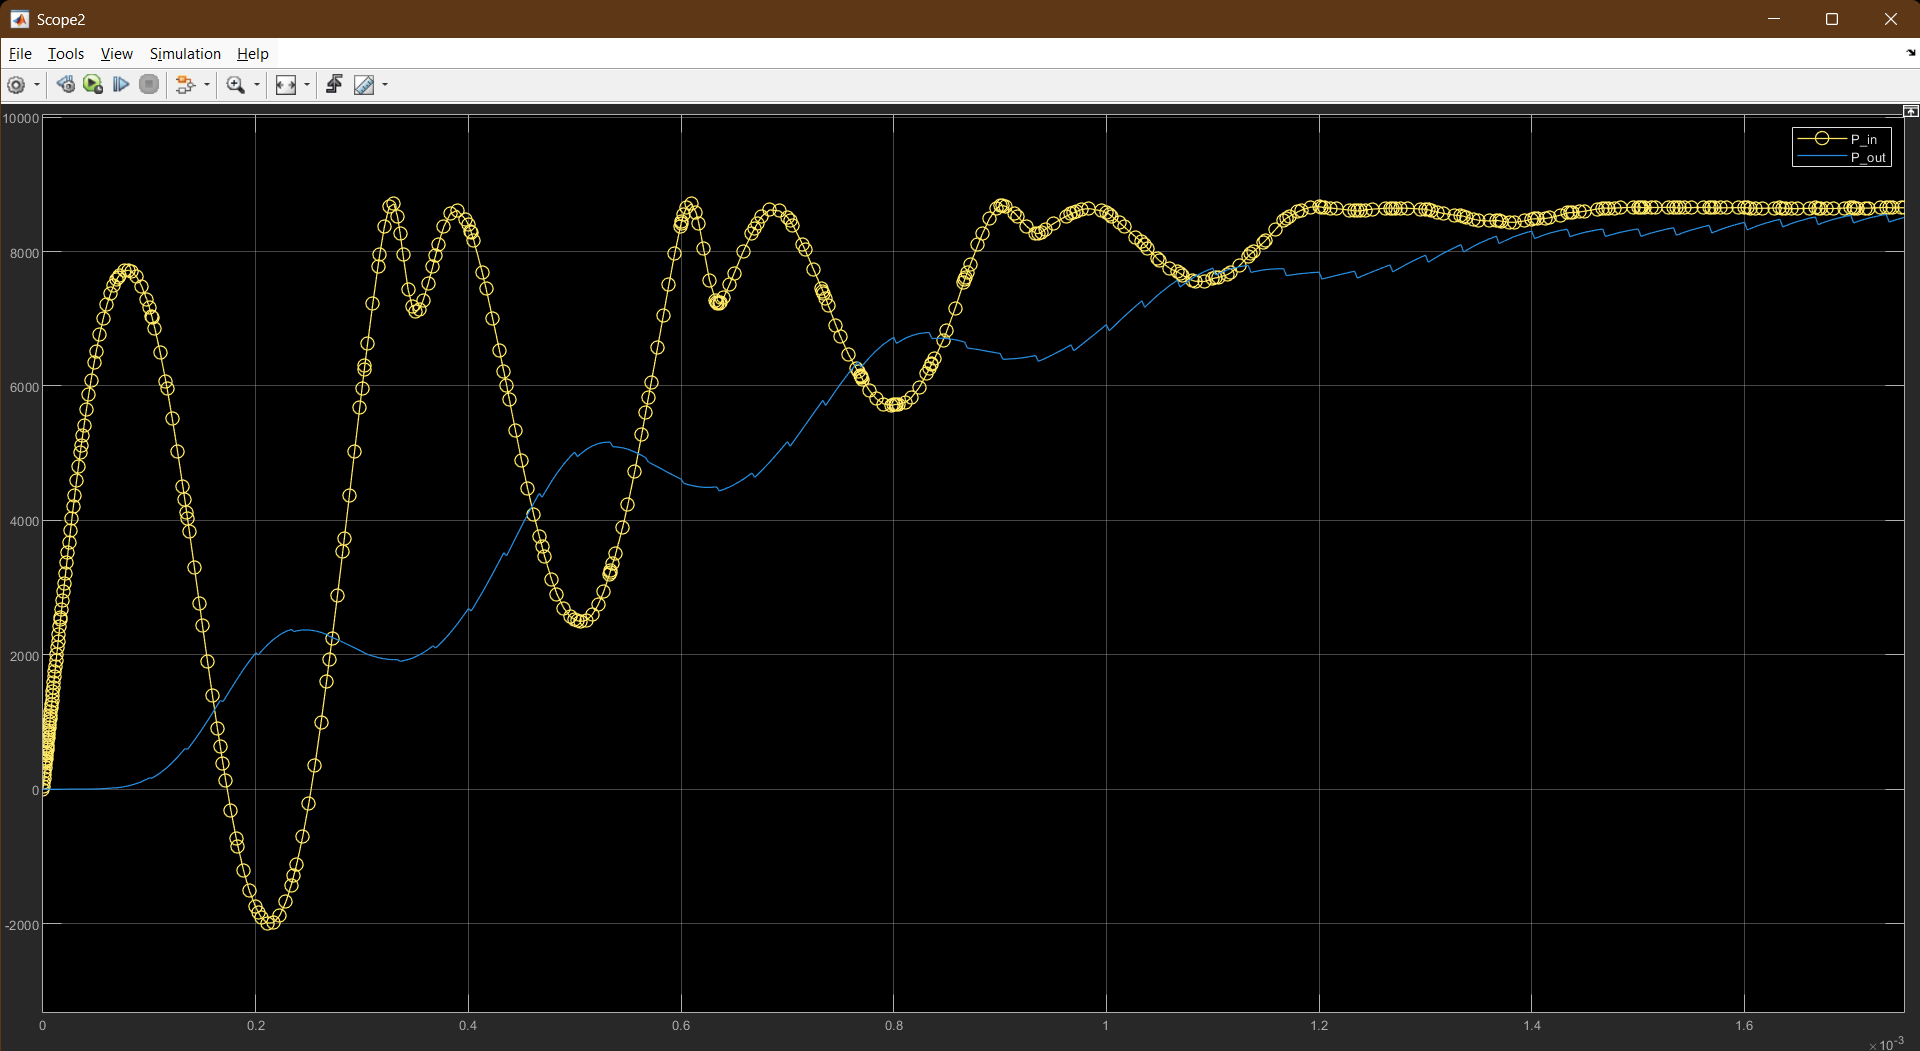
\includegraphics[width=0.9\linewidth]{fot/Ps.png} % ajustar ancho si es necesario
    \caption{La curva amarilla muestra la \textbf{potencia instantánea} ($P_{in}$) entregada por un arreglo de 6 paneles en serie y 6 en paralelo, bajo una \textbf{irradiancia constante} de $1000 \, \text{W/m}^2$ y una \textbf{temperatura} de $25^\circ C$. La curva azul muestra la \textbf{potencia instantánea} ($P_{out}$) entregada a la carga bajo las mismas condiciones. El modelo de panel utilizado es el \textbf{\_A10J\_M60\_240}.}
    \label{fig:Ps}
\end{figure}

---

\begin{figure}[ht!]
    \centering
    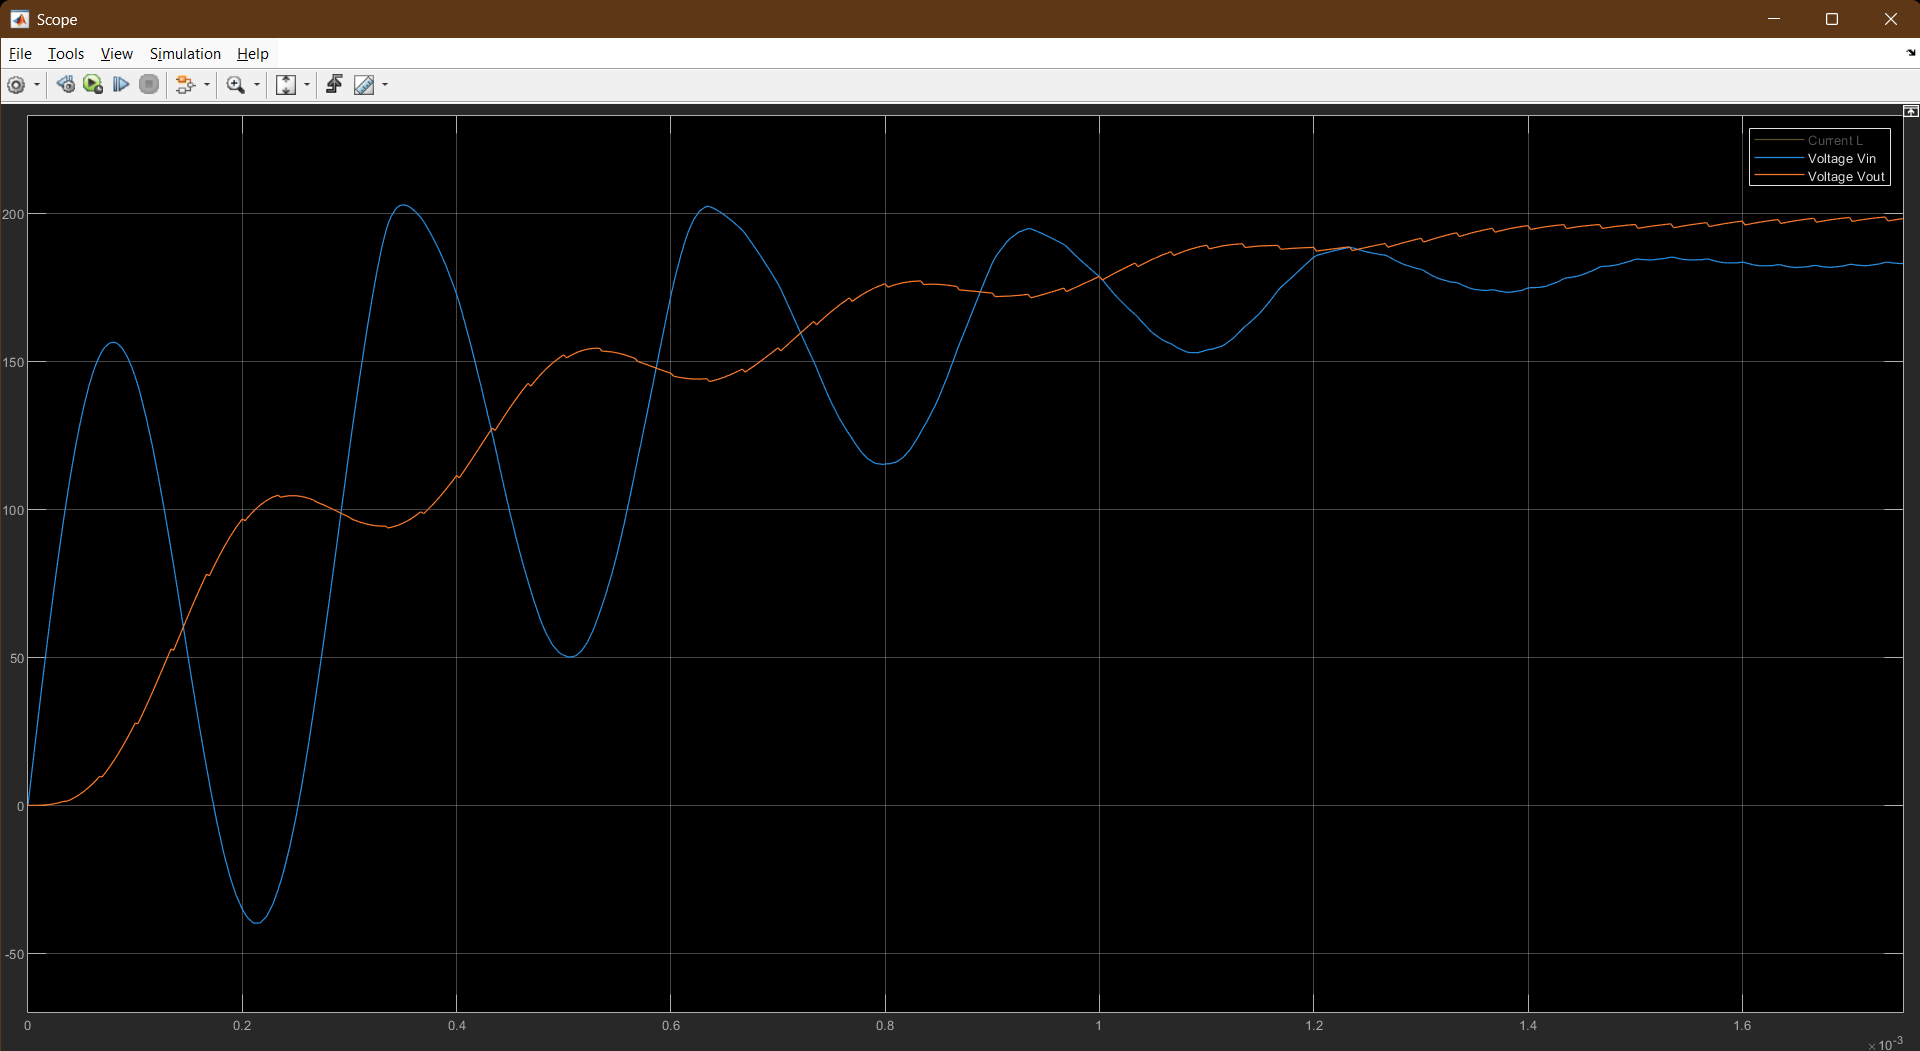
\includegraphics[width=0.9\linewidth]{fot/Vs.png} % ajustar ancho si es necesario
    \caption{La curva azul muestra la \textbf{tensión} ($V_{in}$) entregada por el arreglo de paneles, con el ciclo de trabajo y la distribución mencionados previamente. La curva naranja muestra la \textbf{tensión} ($V_{out}$) en la carga final.}
    \label{fig:Vs}
\end{figure}


\section*{Conclusiones}
\begin{itemize}
\item En base a la práctica de laboratorio realizada, se pudo comprobar mediante el diseño la importancia del adecuado dimensionamiento de los componentes del convertidor para garantizar un funcionamiento estable del sistema fotovoltaico. Los resultados arrojados por la simulación de Simulink concuerdan con los valores hallados teóricamente.

\item De la Figura \ref{fig:simulacion_pv} cabe resaltar que es a una irradiancia constante, sin embargo se podria analizar el sistema control MPPT en el convertidor boost para un vector de irradiacia en el arreglo PV, con el fin de representar como cambian las condiciones de operacion y que se este siguiendo el punto de maxima potencia.
\end{itemize}

\nocite{*} %incluye todas las referencias del .bib aunque no se citen en el texto
\bibliographystyle{IEEEtran}
\bibliography{1}

\end{document}